\section{Quotes from literatures --- Argon momentum transfer}

\subsubsection{Biagi}
A comment from Biagi in \cite{Pitchford2013}:
\blockquote{
The measurements at the Ion Diffusion Unit at Australian
National University (see for example, \cite{Robertson1977})
showed that the sensitivity of the measurements drift
velocity to impurities can be large. For drift velocities,
I propose that the best choice is to exclude data before
the late 1960s as the measurements were done with
up to $20ppm$ of impurities in the gases. The drift
velocity measurements are the best test of cross sections
measurements since they are the most accurate. Thus, we
limit the comparisons to measurements to those with $\pm1\%$
statistical and systematic errors or better where possible.
}
Comments in \cite{Pitchford2013} related to Biagi:
\blockquote{
The cross section sets for argon in both of these databases
were derived from fitting to accurate drift velocity and
diffusion measurements using double shutter drift tubes with
variable drift distances (Nakamura~\cite{Nakamura1988}).
($\ldots$)
At higher values of E/N, the drift velocity measured by
Nakamura~\cite{Nakamura1988} is taken as the most accurate
and both cross section sets fit well to these measurements with
less than $1\%$ deviations on average.
($\ldots$)
In the
original derivation of the set 7.1 we used compatible values
of the $s$-state cross sections to those used by~\cite{Nakamura1988} and as a result we obtained and used a similar elastic
momentum-transfer cross section above $1.0 eV$.\\
It became apparent after the publications of \cite{Allan2006}
that the cross sections for the s-states close to threshold
were much higher than were used in the version 7.1 dataset.
This fact and the need to model more accurately the light
emission from excimers (\cite{Oliveira2011}) and the Penning
transfers in argon gas mixtures (\cite{Sahin2010}) led to the
development of the cross section set 8.9 with a more accurate
description of the level structure. The momentum-transfer
cross section at the peak in version 8.9 is slightly higher than
in 7.1 in order to compensate for the different excitation cross
section.
}
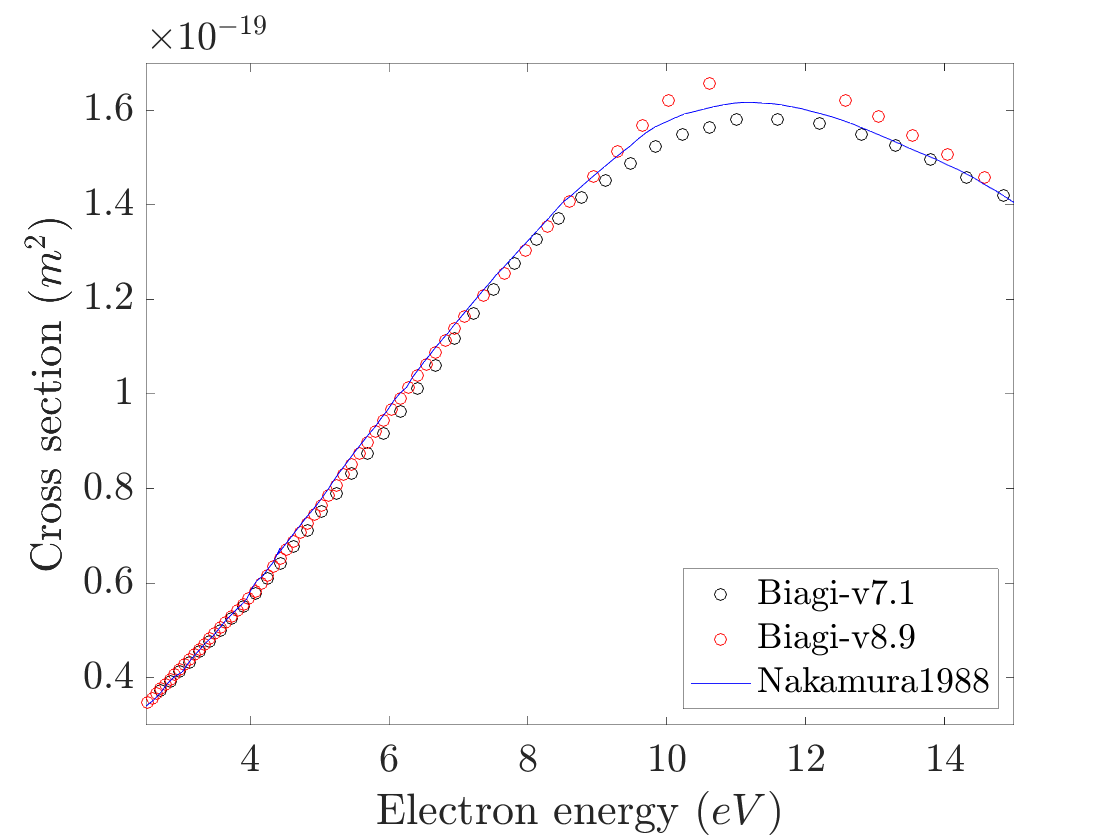
\includegraphics[width=0.5\textwidth]{./figures/collision_dependency}

Followings are the details of Nakamura~\cite{Nakamura1988}.
\begin{itemize}
\item Experiment: double shutter drift tube~\cite{Nakamura1987}
\item Measurement: drift velocity ($W$) and longitudinal diffusion coefficient (times number density, $ND_L$) of electron
\item Measurement error
\begin{itemize}
\item Drift velocity: maximum possible error $2\%$, typical standard deviation less than $1\%$
\item Longitudinal diffusion coeff. (presumably $ND_L$): maximum possible error $10\%$, typical error not specified ("larger scatter")
\end{itemize}
\item Numerically solved the equation (2-4) in \cite{Lowke1969}. Used a backward integration procedure using the Runge--Kutta method. See \cite{Parker1969,Lowke1969,Frost1962}\\
%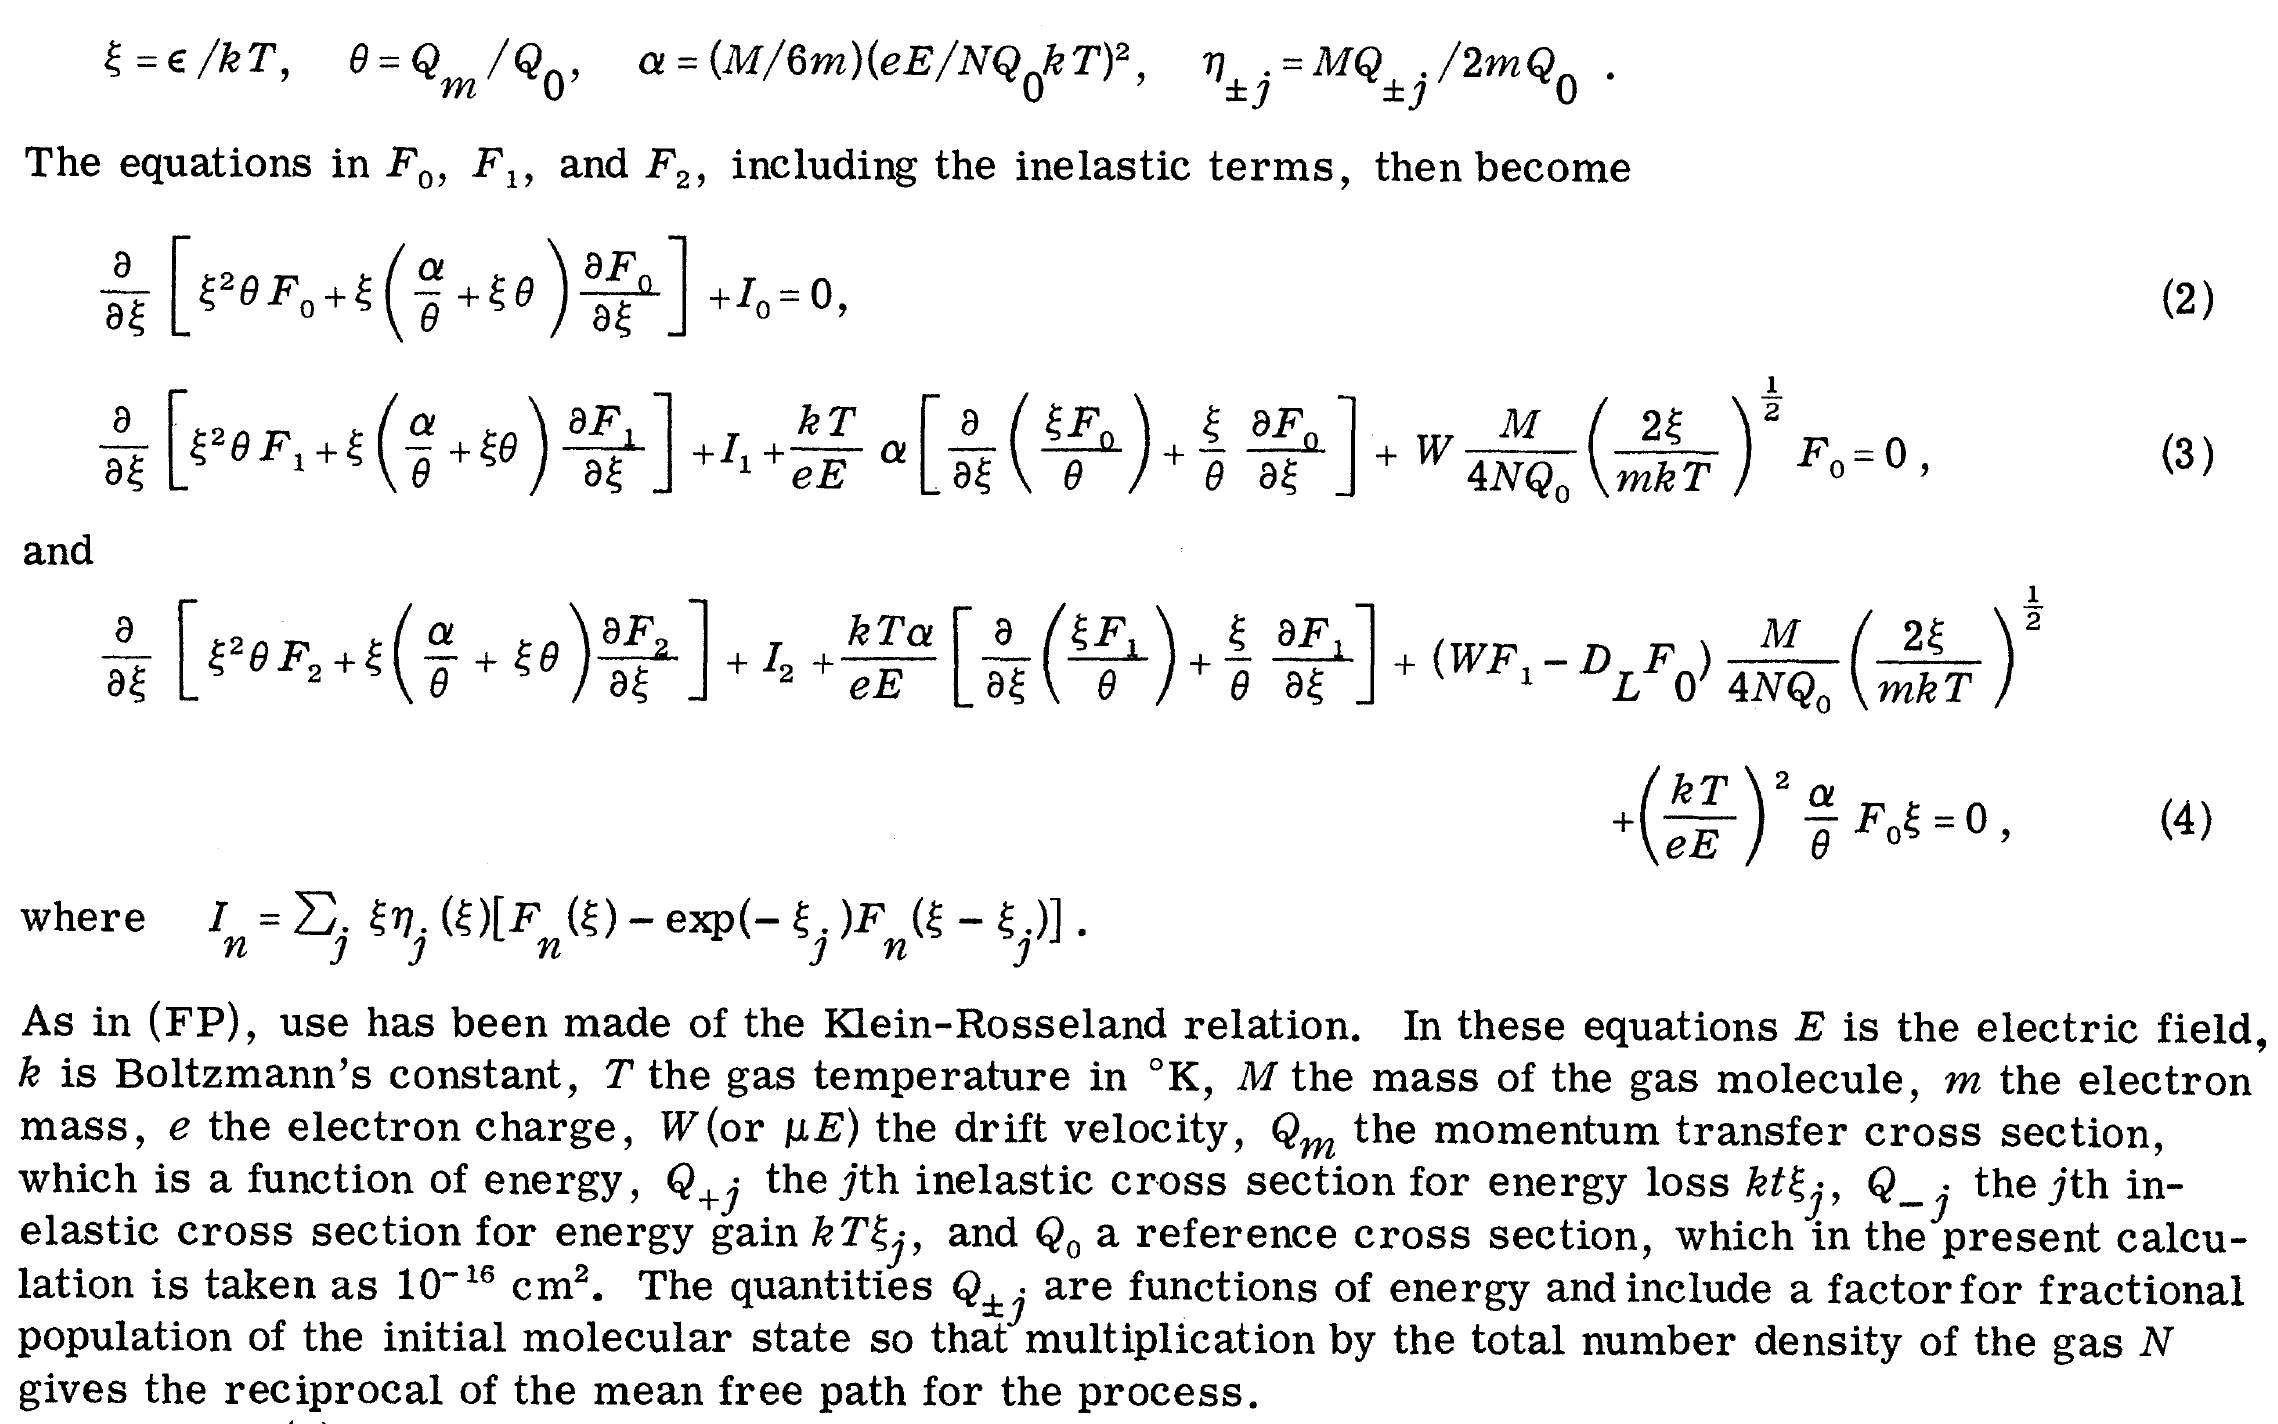
\includegraphics[width=1.0\textwidth]{./figures/lowke1969-eq234}
\item The analysis above focused on the range of electron energy $2.5eV$ to $15eV$,
and other sets of collision cross sections are combined:
\begin{itemize}
\item $\le2.5eV$: \cite{Milloy1977}
\item $\ge15eV$: \cite{Fon1983}
\item Excitation cross section: \cite{Ferreira1983}
\item Ionization cross section: \cite{Rapp1965}
\end{itemize}
\item Resulting drift/diffusion property from the ``derived" cross section\\
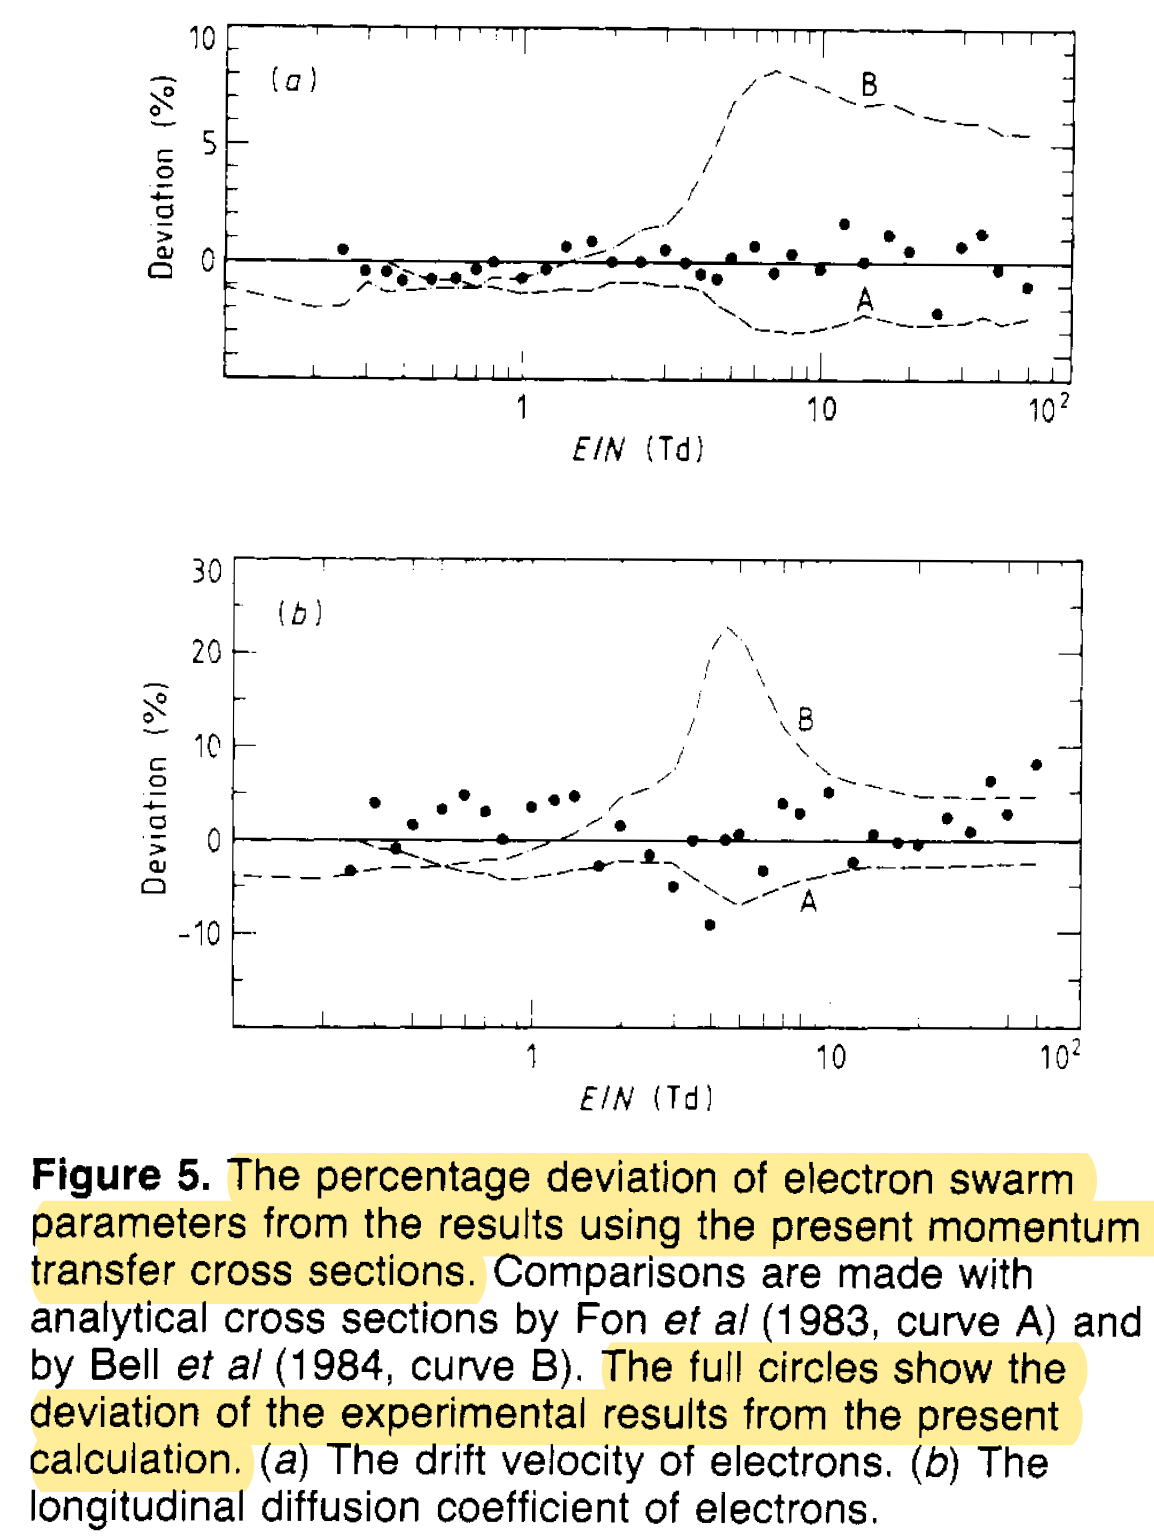
\includegraphics[width=0.6\textwidth]{./figures/nakamura1988-fig5}
\end{itemize}

\subsubsection{BSR-500}

Comments from \cite{Zatsarinny2014}:
\blockquote{
Over the years,
several experiments have been carried out and many other
calculations were performed for comparison. Many of the
numerical models were designed to treat elastic scattering
and hence it is not surprising that the overall agreement
between experiment and theory is generally satisfactory (see,
for example, [1] for detailed comparisons and also Fig. 2
below). It is however worth noting that our BSR approach can
handle the entire energy range with a single approach, which
is also used to treat the excitation and ionization processes
discussed in the following subsections.
}

Comments in \cite{Pitchford2013} related to BSR:
\blockquote{
We believe the elastic and momentum-transfer cross
sections to be accurate at the level of a few per cent. This
assessment is supported by the excellent agreement seen
in this paper between modeling predictions using these
cross sections and the corresponding experimental data.
}

Pseudo states approximation in BSR~\cite{Zatsarinny2013}:
\blockquote{
The use of `pseudo-orbitals' and `pseudo-states' constructed
with at least one of these orbitals being in a dominant
configuration has a long history in atomic structure and
collision calculations. Generally speaking, their role is
twofold: they can be used to account for (i) the term
dependence of the physical orbitals and (ii) the coupling to
the ionization continuum.
}

\subsubsection{Hayashi}
\begin{itemize}
\item Reference: \cite{Pitchford2013,Pitchford2017,Hayashi2003}
\item Compilation of 1960 references
\item ($\ldots$) The cross sections were determined from available data from electron beam and
electron swarm experiments via the Boltzmann equation and
the Monte Carlo simulation method. The beam data were given
highest priority, and theoretical values of cross sections were
sometimes used.
\item Error magnitude is not provided
\end{itemize}

\subsubsection{IST-Lisbon}
\begin{itemize}
\item LXCat reference: \cite{Pitchford2013,Pitchford2017,Alves2014}
\item \cite{Pitchford2017}\\
For each gas the database presents a complete set of cross sections,
validated against measured swarm parameters by solving
the two-term homogeneous electron Boltzmann equation.
In most cases, predictions are in agreement with
measurements within $1\sim20\%$, for reduced electric fields
$E/N = 10^{-4} \sim 500 Td$.
\item \cite{Pitchford2013}\\
The compilation and adjustment of our complete set of
electron-neutral scattering cross sections from ground-state
argon is reported in the following work: (Yanguas-Gil~\cite{Alves2005}).
This paper presents detailed comparisons between
our final set of cross sections and the ones proposed by other authors.
The elastic momentum-transfer cross section was
obtained from Phelps ftp://jila.colorado.edu/collision-data/
electronneutral/electron.txt (Yamabe~\cite{Yamabe1983}).
\item \cite{Alves2014}\\
In general, our cross sections yield predictions for the electron transport parameters and rate coefficients,
calculated with a two-term Boltzmann solver, which agree within less than $20\%$ with measurements,
for reduced electric fields $E/N=10^{-4}\sim 500Td$.
\item \cite{Alves2014}\\
$\ldots$ The compilation and adjustment of the complete set of electron–neutral scattering cross sections from
ground-state argon is reported in~\cite{Alves2005}. The set includes 39 cross sections (elastic momentum-transfer,
37 excitations and ionization) up to 1 keV.\\
$\ldots$ The elastic momentum-transfer cross section was obtained from~\cite{Yamabe1983}.
\item \cite{Alves2005} --- The updated set is
validated by comparing calculated swarm parameters and rate coefficients
(obtained by solving the two-term approximation electron Boltzmann
equation) with available experimental data.\\
$\ldots$ This work follows the recommendations of Phelps and
co-workers, adopting a total momentum transfer cross section
$\sigma_m$ that includes the elastic contribution $\sigma_{m,el}$ proposed by
\cite{Phelps1997} and by~\cite{Yamabe1983}, and the
total inelastic contribution calculated (for coherency) from the
cross section set adopted here, $\sigma_m = \sigma_{m,el} + \sigma_{t,exc} + \sigma_{ion}$.\\
$\ldots$ Simulation results for the electron drift velocity and
characteristic energy were found to be in very good agreement
with experimental values of these quantities, which only
confirms the correct choice of the elastic momentum transfer
cross section proposed by Phelps~\cite{Phelps1997} and Yamabe~\cite{Yamabe1983}.
\item Phelps database from LXCat does not have elastic momentum transfer.
It includes effective momentum transfer, which seems to be the equation above $\sigma_m = \sigma_{m,el} + \sigma_{t,exc} + \sigma_{ion}$.
Elastic momentum transfer from IST-Lisbon is identical to this effective cross section for $\le10eV$ (figure below).\\
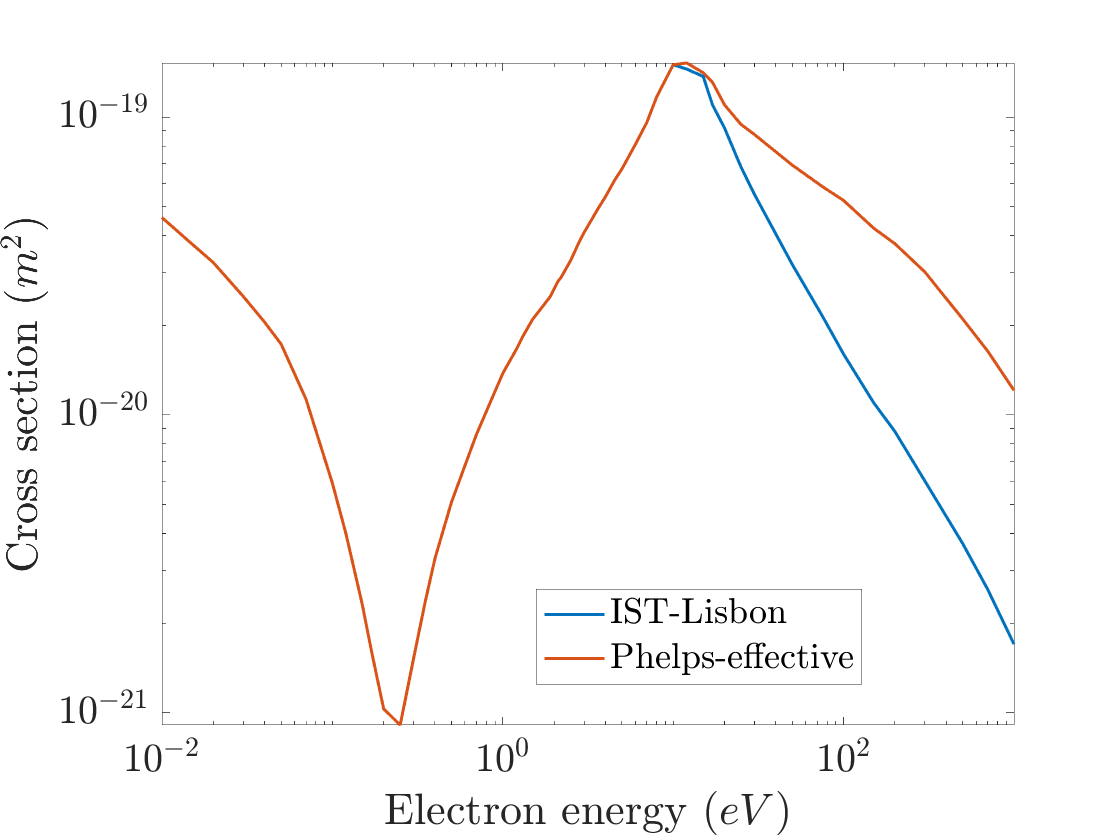
\includegraphics[width=0.6\textwidth]{./figures/ist-phelps}
\end{itemize}

\subsubsection{Phelps}
\begin{itemize}
\item Reference: \cite{Pitchford2013,Pitchford2017}
\item \cite{Pitchford2013}\\
The original version of the cross section set available at
LXCat was based on Frost and Phelps~\cite{Frost1964} as modified
in Tachibana and Phelps~\cite{Tachibana1981}.\\
\begin{itemize}
\item momentum transfer for $<4eV$: Milloy et al~\cite{Milloy1977}
\item momentum-transfer for $>8eV$: Fletcher and Burch~\cite{Fletcher1972}
\item total excitation cross section: Schaper and Scheibner~\cite{Schaper1969}
\item ionization cross section: Smith~\cite{Smith1930}
\end{itemize}
\item \cite{Pitchford2013}\\
The cross section set available at LXCat has been tested
through the comparison of calculated transport and reaction
rate coefficients with experiment in pure Ar for $1\le E/N \le 3000Td$.
Only the very early comparison with experiment in Frost and Phelps~\cite{Frost1964}
got published.
\item $O_2$ property measurement in $Ar-O_2$ mixture \cite{Tachibana1981}\\
Calculations using these cross section sets are found to yield electron attachment
coefficients in agreement with experiment to within experimental
uncertainty. Similarly, calculated electron drift velocities agree with measured values to within
$10\%$ for the $E/N$ range of our experiments.
\item The dataset is derived for use with the two-term
spherical harmonic expansion technique for solving the
electron Boltzmann equation.
\item Nakamura~\cite{Nakamura1988}, which similar to Biagi,
also used cross section of Milloy et al~\cite{Milloy1977}.
Figure below shows the similiarity of Biagi, Phelps to Milloy.\\
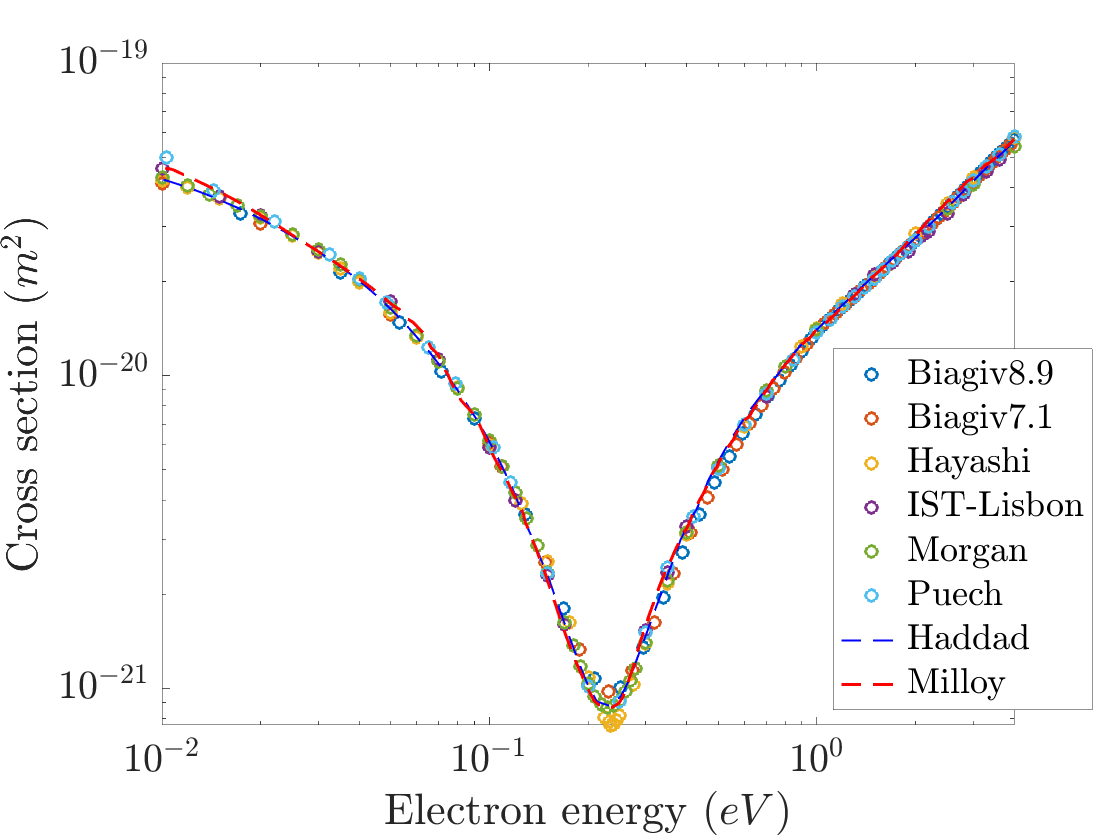
\includegraphics[width=0.6\textwidth]{./figures/milloy}
\end{itemize}

\subsubsection{Morgan}
\begin{itemize}
\item \cite{Pitchford2017}\\
For a wide variety of applications and starting in the mid-1970’s,
WL Morgan compiled the sets of electron scattering
cross sections in this database. $(\ldots)$
There is some overlap with datasets in the Phelps and Hayashi databases on LXCat
which is retained simply so that users can recover previously used data.
\item Not sure the sentence above corresponds to Ar.
Comparison with Phelps (IST-Lisbon) and Hayashi is shown below:\\
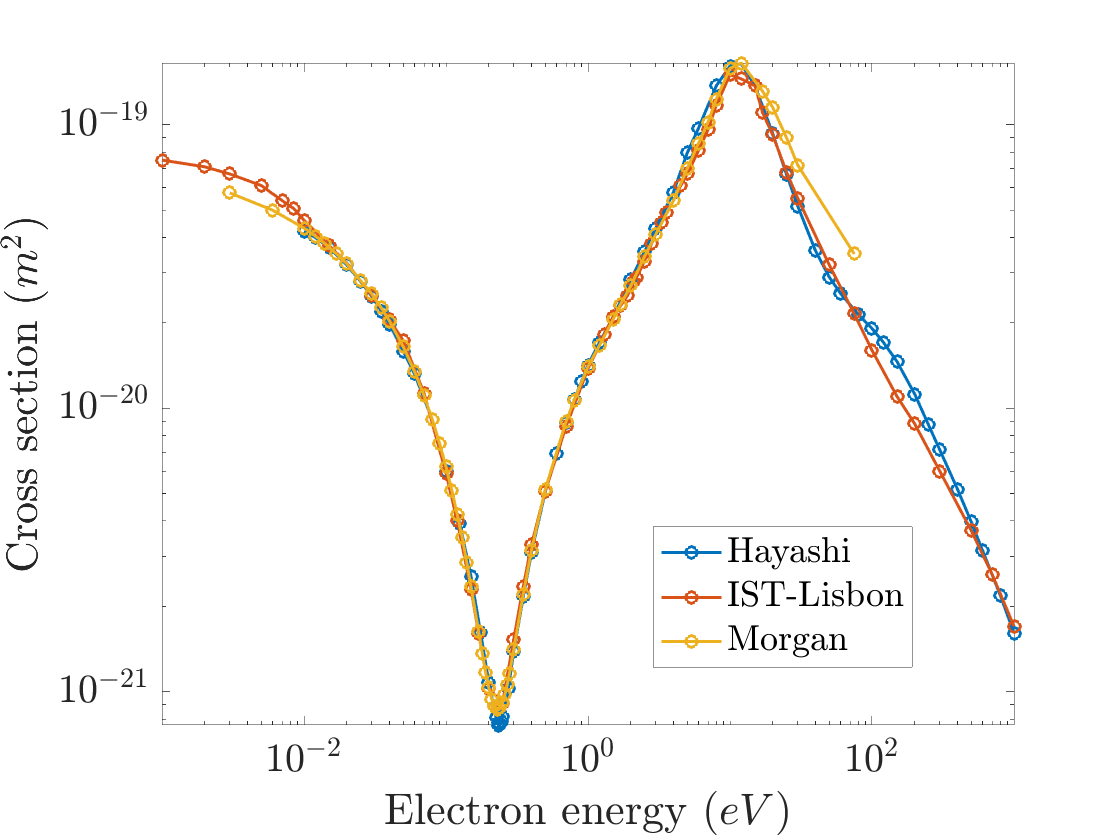
\includegraphics[width=0.6\textwidth]{./figures/morgan}
\item \cite{Pitchford2017}\\
One point to note is that the rotational excitation is
treated using a continuous approximation for rotation
(CAR) that is described by Frost and Phelps~\cite{Frost1962} and by
Morgan and Penetrante. The value of CAR is given in the
datasets but is not used in the on-line Boltzmann solver.
Thus, caution should be exercised in the interpretation of
the on-line calculations of swarm parameters at low $E/N$
where rotational excitation/deexcitation can have an
influence.
\item \cite{Pitchford2013}\\
The details of how Morgan’s data in noble gases were
compiled cannot be recalled at this point. However, the
procedure was standard: a choice was made about the level
of detail to be included for excitation (in this case, two
excited levels to represent allowed and forbidden transitions),
cross sections were estimated or guessed based on experiment
and theory, and then these cross sections were adjusted by
comparing measured swarm parameters with those calculated
using ELENDIF, Morgan’s two-term Boltzmann code (Morgan
and Penetrante 1990).
\item \cite{Pitchford2013}\\
The maximum energy in the data table or the elastic
momentum-transfer cross section in the Morgan database
is $75 eV$ and it is lower in the heavier noble gases. The
calculations reported here were done using the default
extrapolation scheme in BOLSIG+ assuming that cross
sections for energies higher than the last entry in the tables
decrease like $\log(\epsilon)/\epsilon$ where $\epsilon$ is electron energy, consistent
with the high-energy limit for cross sections for allowed
transitions in the Born approximation.
\end{itemize}

\subsubsection{Puech}
\begin{itemize}
\item Reference: \cite{Pitchford2013,Puech1986}
\item \cite{Pitchford2013}\\
The article by Puech and Torchin~\cite{Puech1986} describes in detail
the procedure used for the compilation and consistency
checking of this cross section set by comparisons with selected
experiments.
\item \cite{Puech1986}\\
we use an appropriate code which solves the Boltzmann equation in the usual two-term spherical
harmonic expansion.
\item \cite{Puech1986}\\
For elastic processes, we have used the momentum transfer cross section
given by Frost and Phelps~\cite{Frost1964} except in the range
$0.014-4eV$ where we have adopted the data of Milloy~\cite{Milloy1977}.
In LXCat databases, Puech seems to be interpolated between these two literatures.
For $<0.014eV$, data seems to be extrapolated.\\
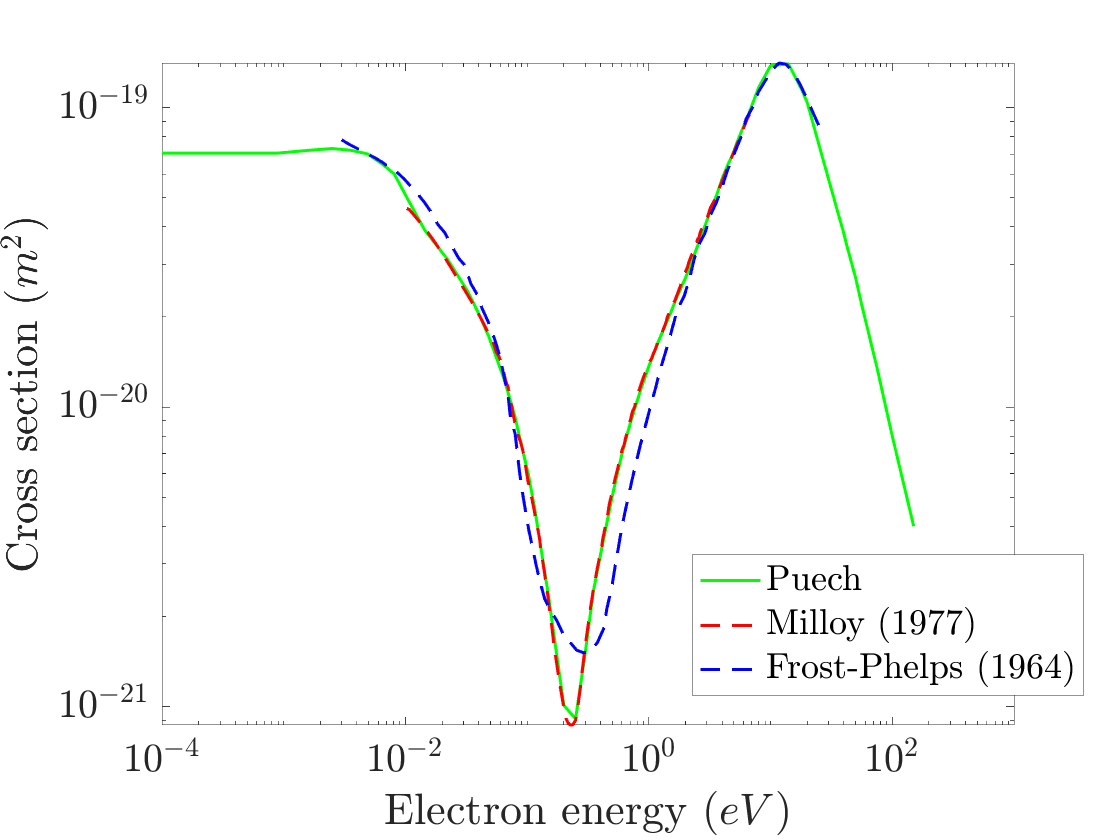
\includegraphics[width=0.6\textwidth]{./figures/puech}
\item Like other Boltzmann analysis, a set of cross sections are chosen from different literatures,
and compared the swarm parameters.
\item \cite{Pitchford2017}\\
Calculations of swarm parameters were made using a two-term Boltzmann
solver as well as the multiterm solver developed by
S\'{e}gur and Bordage~\cite{Segur1989}.
\end{itemize}